\documentclass[aspectratio=43,english]{beamer} %If you want to create Polish presentation, replace 'english' with 'polish' and uncomment 3-th line, i.e., '\usepackage{polski}'
\usepackage[utf8]{inputenc}
\usepackage{polski} %Uncomment for Polish language
\usepackage{babel}
\usepackage{listings} %We want to put listings

\mode<beamer>{ 	%in 'beamer' mode
	\hypersetup{pdfpagemode=FullScreen}		%Enable Full screen mode
	\usetheme{JuanLesPins} 		%Show part title in right footer
	%\usetheme[dark]{AGH}                 		%Use dark background
	%\usetheme[dark,parttitle=leftfooter]{AGH}  	%Use dark background and show part title in left footer
}
\mode<handout>{	%in 'handout' mode
	\hypersetup{pdfpagemode=None}		
	\usepackage{pgfpages}
  	\pgfpagesuselayout{4 on 1}[a4paper,border shrink=5mm,landscape]	%show 4 slides on 1 page
  	\usetheme{boxes}
  	\addheadbox{structure}{\quad\insertpart\hfill\insertsection\hfill\insertsubsection\qquad} 	%content of header
 	\addfootbox{structure}{\quad\insertauthor\hfill\insertframenumber\hfill\insertsubtitle\qquad} 	%content of footer
}

\AtBeginPart{ %At begin part: display its name
	\frame{\partpage}
} 


%%%%%%%%%%% Configuration of the listings package %%%%%%%%%%%%%%%%%%%%%%%%%%
% Source: https://en.wikibooks.org/wiki/LaTeX/Source_Code_Listings#Using_the_listings_package
%%%%%%%%%%%%%%%%%%%%%%%%%%%%%%%%%%%%%%%%%%%%%%%%%%%%%%%%%%%%%%%%%%%%%%%%%%%%
\lstset{ %
  backgroundcolor=\color{white},   % choose the background color
  basicstyle=\footnotesize,        % the size of the fonts that are used for the code
  breakatwhitespace=false,         % sets if automatic breaks should only happen at whitespace
  breaklines=true,                 % sets automatic line breaking
  captionpos=b,                    % sets the caption-position to bottom
  commentstyle=\color{green},      % comment style
  deletekeywords={...},            % if you want to delete keywords from the given language
  escapeinside={\%*}{*)},          % if you want to add LaTeX within your code
  extendedchars=true,              % lets you use non-ASCII characters; for 8-bits encodings only, does not work with UTF-8
  frame=single,	                   % adds a frame around the code
  keepspaces=true,                 % keeps spaces in text, useful for keeping indentation of code (possibly needs columns=flexible)
  keywordstyle=\color{blue},       % keyword style
  morekeywords={*,...},            % if you want to add more keywords to the set
  numbers=left,                    % where to put the line-numbers; possible values are (none, left, right)
  numbersep=5pt,                   % how far the line-numbers are from the code
  numberstyle=\tiny\color{gray},   % the style that is used for the line-numbers
  rulecolor=\color{black},         % if not set, the frame-color may be changed on line-breaks within not-black text (e.g. comments (green here))
  showspaces=false,                % show spaces everywhere adding particular underscores; it overrides 'showstringspaces'
  showstringspaces=false,          % underline spaces within strings only
  showtabs=false,                  % show tabs within strings adding particular underscores
  stepnumber=2,                    % the step between two line-numbers. If it's 1, each line will be numbered
  stringstyle=\color{cyan},        % string literal style
  tabsize=2,	                   % sets default tabsize to 2 spaces
  title=\lstname,                  % show the filename of files included with \lstinputlisting; also try caption instead of title
                                   % needed if you want to use UTF-8 Polish chars
  literate={?}{{\k{a}}}1
           {?}{{\k{A}}}1
           {?}{{\k{e}}}1
           {?}{{\k{E}}}1
           {�}{{\'o}}1
           {�}{{\'O}}1
           {?}{{\'s}}1
           {?}{{\'S}}1
           {?}{{\l{}}}1
           {?}{{\L{}}}1
           {?}{{\.z}}1
           {?}{{\.Z}}1
           {?}{{\'z}}1
           {?}{{\'Z}}1
           {?}{{\'c}}1
           {?}{{\'C}}1
           {?}{{\'n}}1
           {?}{{\'N}}1
}
%%%%%%%%%%%%%%%%%


\title{Metody Obliczeniowe w Nauce i Technice}
\author{Marian Bubak, PhD}
\date{}
\institute[AGH]{
	Institute of Computer Science\\ul. Kawiory 21\\30-055 Krakow\\
	Poland\\
	\url{http://www.icsr.agh.edu.pl/~mownit/}
}


\usepackage{amsmath}
\usepackage{mathtools}
\usepackage{graphicx}

\subtitle{20 - Wprowadzenie do metody różnic skończonych}
\begin{document}
  	\maketitle
	%%%%%%%%%%%%%%%%
	\begin{frame}{Outline}
		\tableofcontents
	\end{frame}
	%%%%%%%%%%%%%%%%
	\section{Wstęp}
\begin{frame}{Wstęp}
	\begin{exampleblock}{}
		 \[
    	\textrm{Analiza matematyczna - obiekty}
        \begin{cases}
        	\textrm{nieskończone} \\
            \textrm{ciągłe}
        \end{cases}
    	\] 
    	$\newline$
    	\[
    	\textrm{Arytmetyka komputerowa}
        \begin{cases}
        	\textrm{skończona} \\
            \textrm{dyskretna}
        \end{cases}
    	\]
	\end{exampleblock}
\end{frame}
\begin{frame}{Cel i sposób}
	\begin{block}{Cel:}
		Przełożenie równań procesów fizycznych na język arytmetyki 
    	komputerowej
	\end{block}
    \begin{block}{Sposób:}
     	Metoda różnic skończonych ($\rightarrow$ małe elementy ciągłego układu fizycznego) $\newline$
        \textbf{Istota:} zatrzymanie się na pośrednim etapie $\newline$
        na drodze do równań różniczkowych $\rightarrow$
        układy równań różniczkowych
        \[	\textrm{zmienne ciągłe}
        	\begin{rcases*}
        		\nearrow \textrm{czasowe - t} \\
                \searrow \textrm{przestrzenne - x}
        	\end{rcases*}
        	\rightarrow siatka
            \begin{cases}
            	\textrm{czasowa} \\
                \textrm{przestrzenna}
            \end{cases}
        \]
    \end{block}
     
\end{frame}
	%%%%%%%%%%%%%%%%%%%%%%%
\section{Reprezentacja dyskretnej zmiennej ciągłej}
\begin{frame}{Reprezentacja dyskretnej zmiennej ciągłej - zmienna}

	
	\begin{minipage}{0.6\textwidth}\raggedright
		x - ciągła zmienna niezależna \\
        $X_{1} \leq x \leq X_{2}$ \\ 
        $\newline \newline$
        siatka(przestrzenna) punktów: \\
        $1 \leq j \leq J \rightarrow \textrm{węzły siatki}$ \\
        $\Delta x_{j}$ - kroki siatki
        \\
        $\newline \newline$
        $x \rightarrow \{ x_{j} \}$ \\
        zmienna ciągła $\rightarrow$ wektor o wymiarze J
        
	\end{minipage}
    \hfill%
    \begin{minipage}{0.385\textwidth}
		%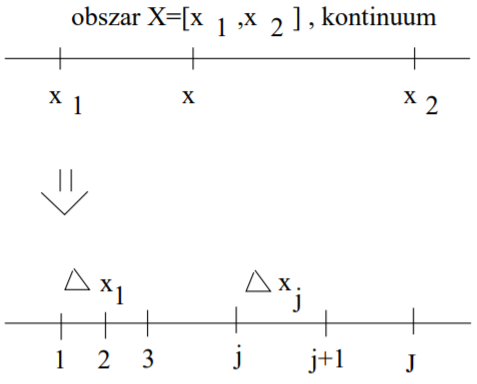
\includegraphics[width=\linewidth]{img/20/mrs_img_1}
        \begin{figure}[t]
			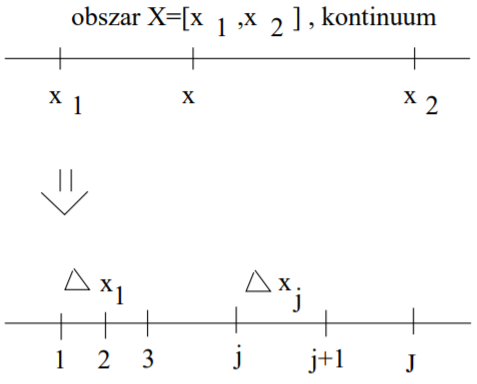
\includegraphics[width=5cm]{img/20/mrs_img_1}
		\end{figure}
	\end{minipage}%
	
\end{frame}
%%%%%%%%%%%%%%%%%%5
\begin{frame}{c.d. - funkcja}
	\[
    	\underbrace{f(x)}_{\substack{\textrm{funkcja określona} \\ 
        \textrm{na kontinuum}}}
        = \underbrace{\{ f_{j}=j(x_{j}) \}}
        _{\substack{\textrm{wektor określony} \\ 
        \textrm{na siatce} \  \{ x_{j} \} }}
    \]
    W dowolnym $x': \ x_{j} \leq x' \leq x_{j+1} \newline$
    $f(x)$ można przybliżyć stosując interpolacje liniową:
    \[
    	\epsilon = \frac{x' - x_{j}}{x_{j+1}-x_{j}}
    \]
    \[
    	f^{*} = \epsilon \cdot f_{j+1} + (1- \epsilon) \cdot f_{j}
    \]
\end{frame}















	%%%%%%%%%%%%%%%%%%%%%%%
	\section{Jakość przybliżania funkcji w metodzie rożnicowej}
\begin{frame}{Jakość przybliżania funkcji w metodzie rożnicowej}
	\begin{figure}[h]
			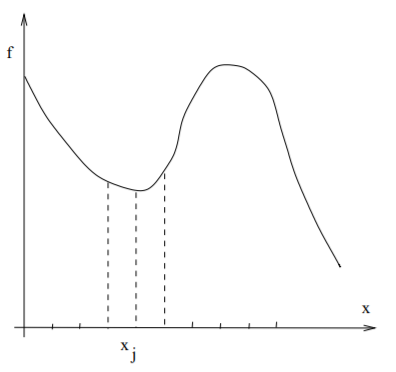
\includegraphics[width=.43\linewidth]{img/20/mrs_img_2}
	\end{figure}
    \begin{exampleblock}{}
    	$\textbf{Dobra:}$ aproksymacja funkcji wolnozmiennej (długofalowej) 
    \end{exampleblock}
    \begin{alertblock}{}
    	$\textbf{Zła:}$ przybliżenie na siatce funkcji szybkozmiennej
    \end{alertblock}
\end{frame}
%%%%%%%%%%%%%%%%%%%%%%%
\begin{frame}
	\begin{figure}[h]
			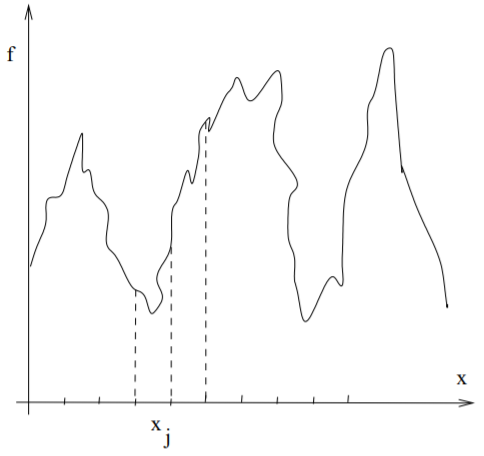
\includegraphics[width=.40\linewidth]{img/20/mrs_img_3}
	\end{figure}
    \newcommand\myeq{\mathrel{\overset{\makebox[0pt]{\mbox{\normalfont\tiny\sffamily (w.Dirichleta)}}}{funkcja}}}
    Opis ilościowy $\rightarrow$ analiza fourierowska:
    $\myeq \ \rightarrow \newline \rightarrow$ ciąg modów Fouriera
    $\newline$f(x):
    \[
    	f(x)=\sum_{l=-\infty}^{\infty}g_{l}\cdot e^{i\cdot k_{l}\cdot x},\
         \ k=\frac{2\pi}{L}\cdot l=k_{0}\cdot l
    \]
    \[
    	g_{l}=\frac{1}{L}\int_{L}dxf(x)e^{-ik_{i}x}
         \ \ 
         \textrm{amplituda fali o długości} \
         \lambda = \frac{L}{l}
    \]
\end{frame}
%%%%%%%%%%%%%%%%%%%%%%%
\begin{frame}
	$\{ f_{j} \}: \ \Delta x =  \Delta$ - stała 
    \[
    	f_{j}=\sum_{l=1}^{J}g_{l}\cdot e^{ik_{l}\cdot x_{j}},\ \ \ k_{l}
        \cdot x_{j}=\frac{2.\pi}{J\cdot \Delta}\cdot l\cdot\Delta
        \cdot j=\frac{2\pi j}{J}
    \]
    \[
    	g_{l}= \frac{1}{L}\sum_{j=1}^{J}f_{j}\cdot e^{ik_{l}\cdot x_{j}} 		\textrm{- amplituda}
    \]
    $\newline$
    Na siatce można opisać tylko skończony zbiór fal, istnieje najmniejsza,
    graniczna długość fali, którą można zdefiniować na siatce:
    $\Delta = \frac{l}{J}$
\end{frame}







	%%%%%%%%%%%%%%%%%%%%%%%
	\section{Pochodne rożnicowe w przestrzeni}
\begin{frame}{Pochodne rożnicowe w przestrzeni}
	\begin{enumerate}
	\item[(a)] $\frac{d}{dx}$ - informacje o lokalnej zmienności funkcji 
    - sprzęga ze sobą sąsiednie węzły siatki $\newline$
    zamiast $\frac{df}{dx} \Bigm|_j \Rightarrow \textrm{aproksymacja:}$
    \[
    	\Delta x'f_{j}=\frac{f_{j+1}-f_{j-1}}{2\cdot\Delta} \ \
        \textrm{("wycentrowana")}
    \]
    jakość aproksymacji - z porównania:
    $
    \begin{cases}
    	\textrm{- pochodnej zwykłej modu Fouriera} \\
        \textrm{- pochodnej różnicowej modu Fouriera}
    \end{cases}
    \newline
    $
    Mod Fouriera: $u=g_{k}\cdot e^{ikx}$
    \[
    	\frac{du}{dx}=ikg_{k}e^{ikx}=ik\cdot u
    \]
	\end{enumerate}
\end{frame}
%%%%%%%%%%%%%%%%%%%555
\begin{frame}
	\begin{figure}[h]
			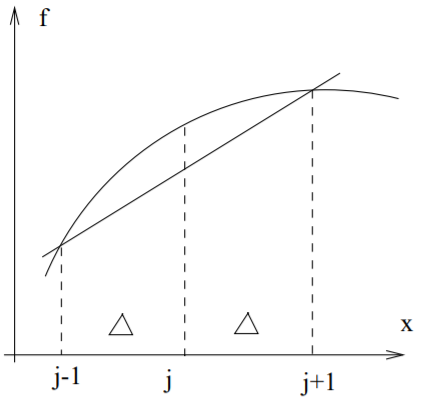
\includegraphics[width=.40\linewidth]{img/20/mrs_img_4}
	\end{figure}
    \[
    	\Delta^{'}_{x}u_{j}=\frac{g_{k}e^{ikx_{j+1}}-
        g_{k}e^{ikx_{j-1}}}{2\cdot\Delta}=\frac{g_{k}e^{ikx_{j}}}
        {2\cdot\Delta}\cdot(e^{ik\Delta}-e^{-ik\Delta})=
    \]
    \[
    	=\frac{i\cdot u}{\Delta}\cdot sin(k\cdot\Delta)=\frac{iu}
        {\Delta}[k\cdot\Delta-\frac{(k\Delta)^{3}}
        {6}+O(k^{5}\Delta^{5})]
    \]
    \[
    	\underbrace{\Delta_{x}'}_{\substack{\textrm{Operator pochodnej} \\ 
        \textrm{różnicowej}}}\ 
        =[1-\frac{(k\Delta)^{2}}{6}+O(k^{4}\Delta^{4})]\ 
        \underbrace{\frac{d}{dx}}_{\textrm{operator pochodnej}}
    \]
\end{frame}
%%%%%%%%%%%%%%%%%%%%%5
\begin{frame}
	Pochodna różnicowa dobrze aproksymuje zwykłą pochodną gdy liczba falowa 
    $k=\frac{2\pi}{L}\cdot l = \frac{2\pi}{\lambda}$ jest mała (dłuższa fala)
    $\newline \newline$
    "wycentrowany" operator $\Delta^{'}_{x}$ - dokładny do wyrazów drugiego 
    rzędu ze względu na $(k \cdot \Delta)^{2}$
\end{frame}
%%%%%%%%%%%%%%%%%%%%%
\begin{frame}
	\begin{enumerate}
    	\item[(b)] $\frac{d^{2}f}{dx^{2}} \rightarrow$ możliwa aproksymacja:
        
	\end{enumerate}
    \begin{figure}[h]
			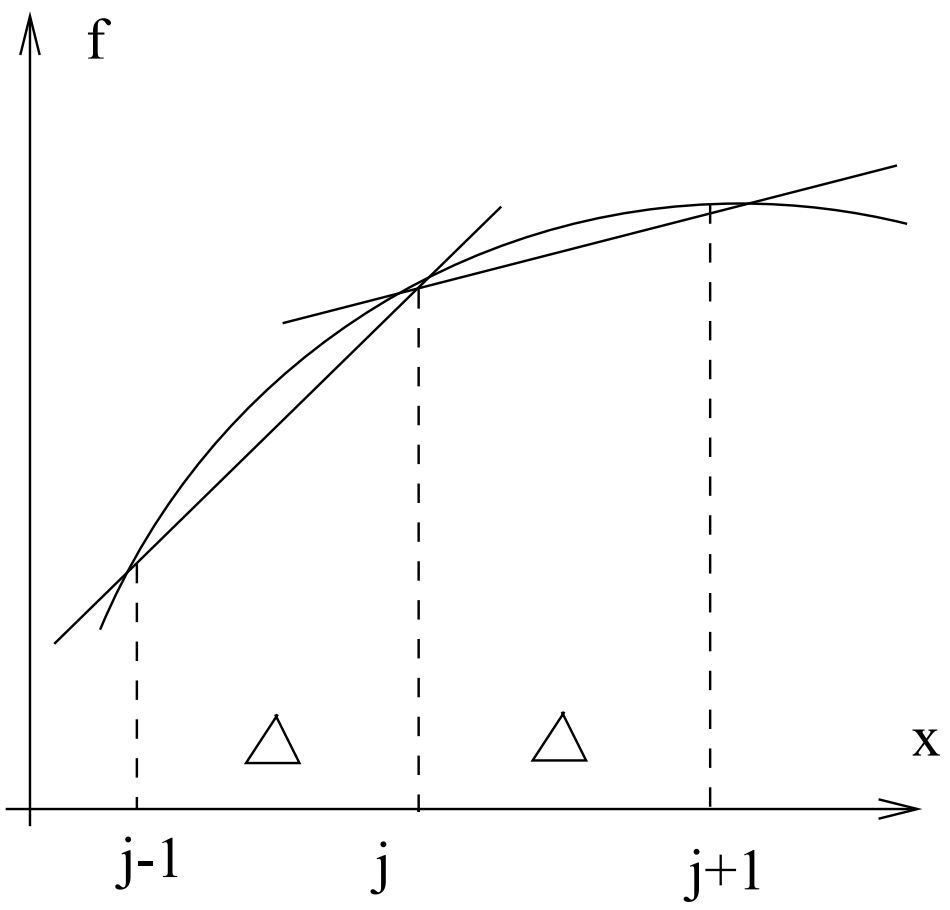
\includegraphics[width=.40\linewidth]{img/20/mrs_img_5}
	\end{figure}
    \[
    	\Delta_{x}''f_{j}=(\frac{f_{j+1}-f_{j}}{\Delta}-\frac{f_{j}-
        f_{j-1}}{\Delta})\cdot\frac{1}
        {\Delta}=\frac{f_{j+1}-2f_{j}+f_{j-1}}{\Delta^{2}}
    \]
    \[
    	\frac{d^{2}u}{dx^{2}}=\frac{d^{2}}{dx^{2}}g_{k}e^{ikx}=-k^{2}\cdot u
    \]
\end{frame}
%%%%%%%%%%%%%%%%%%%%%
\begin{frame}
	\[
    	\Delta{x}''f_{j} = \frac{g_{k}}{\Delta^{2}}
        [e^{ik(x_{j}+\Delta)}-2\cdot e^{ikx_{j}}+e^{ik(x_{j}-
        \Delta)}]=\frac{2u}{\Delta^{2}} [{\it cos} (k\Delta)-1]=
    \]
    \[
    	=\frac{2u}{\Delta^{2}}[1-\frac{k^{2}\Delta^{2}}
        {2}+\frac{k^{4}\Delta^{4}}{24}+O(k^{6}\Delta^{6})-1]=-k^{2}
        u(1-\frac{k^{2}\Delta^{2}}{12}+O(k^{4}\Delta^{4}))
    \]
    \[
    	\underbrace{\Delta_{x}^{''}}_{\substack{\textrm{Operator drugiej} 		\\ 
        \textrm{pochodnej różnicowej}}}\ 
        \ =[1-\frac{k^{2}\Delta^{2}}{12}+O(k^{4}\Delta^{4})]\ 
        \underbrace{\frac{k^{2}}{dx^{2}}}_{\substack{\textrm{Operator 
        drugiej} \\ 
        \textrm{pochodnej}}}
    \]
    $\newline$
    aproksymacja drugiej pochodnej - z dokładnością do wyrazów 2-go rzędu ze
    względu na:
    \[
    	(\frac{2 \pi \cdot \Delta}{\lambda})
    \]
\end{frame}
%%%%%%%%%%%%%%%%%%%%
\begin{frame}{Zastosowanie}
	\begin{block}{}
		Przedstawiona metoda analizy jakości aproksymacji jest przydatna 
        dla:
        \begin{itemize}
        \item pochodnych wyższych rzędow
        \item bardzo złożonych wzorów (operatorów)
        \end{itemize}
	\end{block}
\end{frame}

















	%%%%%%%%%%%%%%%%%%%%%%%
\end{document}
